\documentclass{standalone}

\usepackage{tikz}
\usepackage{circuitikz}
\usetikzlibrary{angles,quotes}
\tikzset{block/.style = {draw, fill=white, very thick, rectangle, minimum height=1cm, minimum width=2cm},
         lblock/.style={draw,fill=white,very thick, rectangle, minimum height=3cm, minimum width=1cm},
         sum/.style= {draw, fill=white, very thick, circle, node distance=0.5cm}}

         
\begin{document}
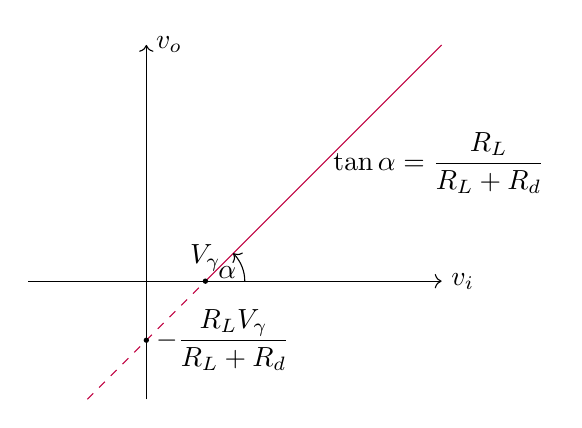
\begin{tikzpicture}[scale=3]
    \draw[->](-0.5,0)--(1.25,0)node[right]{$v_i$};
    \draw[->](0,-0.5)--(0,1)node[right]{$v_o$};

    \draw[purple,dashed](-0.25,-0.5)--(0,-0.25)node[right,black]{$-\displaystyle\frac{R_LV_{\gamma}}{R_L+R_d}$}--(0.25,0)node[above,black]{$V_{\gamma}$};
    \draw[purple](0.25,0)--(1.25,1);
    \coordinate (a) at(0.25,0);
    \coordinate (b) at(1.25,1);
    \coordinate (c) at(1.25,0);
    \filldraw[black](0,-0.25)circle(0.25pt);
    \filldraw[black](0.25,0)circle(0.25pt);
    \node[right] at(0.75,0.5){$\tan\alpha=\displaystyle\frac{R_L}{R_L+R_d}$};
    \pic[draw, ->, black, "$\alpha$", radius=2]{angle=c--a--b};
\end{tikzpicture}
\end{document}